%\section{Matrix Element-based Kinematic Discriminant (\Dkinbkg)}
\section{Matrix Element-based Kinematic Discriminant}
\label{sec:Dkin}
The \Dkinbkg is the last variable that is used to extract the value of \mH.
It is a discriminant sensitive to the kinematical variables of the \qqggzzfourl process and is useful in \emph{discriminating} a signal process from a background process.
% TODO: Define \Dkinbkg.
% TODO: More info in :CITE HIG-19-001.

%\subsection{\Dkinbkg with new muon reconstruction}
%This section will show the possible impact of the new muon reconstruction on the \Dkinbkg.

\subsection{Correlation studies}
\label{sec:DkinCorrelation}
The previous \mH measurement
% TODO:CITE
was obtained assuming no correlation between \relmfourlerrflat and \Dkinbkg.
% TODO: Maybe define relmass4lerr as $D_{m_{4\ell}}$ 
However, \figurename~\ref{Dkin_sigma_correlation} shows $D_{m_{4\ell}} \left( \relmfourlerr \right)$ \vs \Dkinbkg for events that pass full selection, split by final state and by year---a correlation is indeed observed.
Categorizing events by \relmfourlerrflat eliminates this dependence.
\begin{figure}[!htbp]
\begin{center}
	\includegraphics[width=1\textwidth]{../../higgsmassmeasurement/AN-19-248/Figures/BackDiscriminant/CorrelationDkinDRelPlot.pdf}
\caption{$D_{m_{4\ell}}$ \vs \Dkinbkg for different year (in each column) and for different final state (in each row).}
\label{Dkin_sigma_correlation}
\end{center}
\end{figure}

% \subsection{Methodology}
So far, the uncertainties on \mH have been estimated by performing a 1D likelihood fit on \mfourl after implementing the various analysis techniques (Sec.~\ref{sec:techniques}).
To achieve an even lower uncertainty on the final \mH value, a 2D likelihood fit can be performed, incorporating \Dkinbkg into the fit.
The new pdf used to extract the uncertainties on \mH is:
\[
pdf(m'_{4\ell}, \Dkinbkg) = f(m_{4\ell}) \times g(\Dkinbkg, m'_{4\ell}),
\]
for which lepton \pt values have been updated using VX+BS and \Zone refit in each category.

\figurename~\ref{2D_distribution} shows example of the 2D histograms of the g function, for 2018 ggF sample @ 125 \GeV
for different bins and for different final states.
\begin{figure}[!htbp]
\begin{center}
	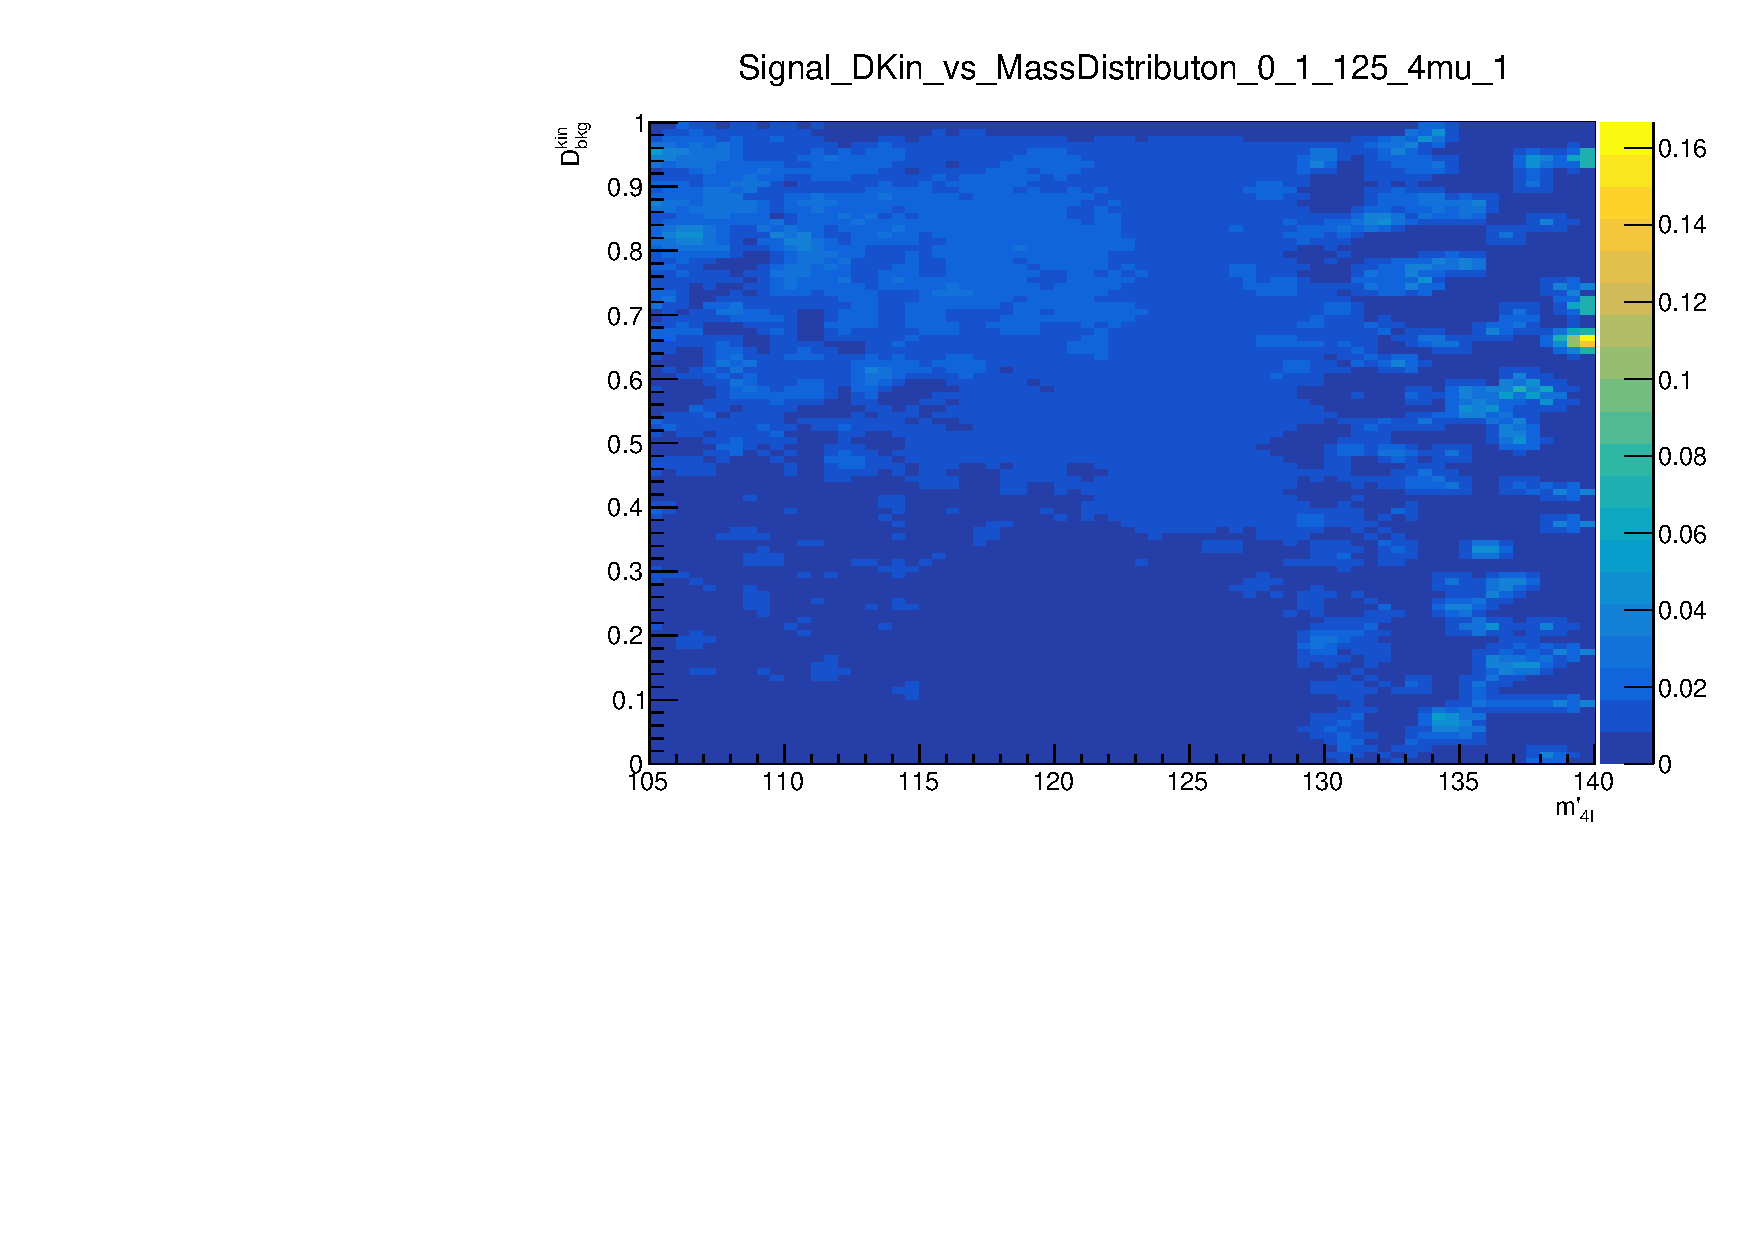
\includegraphics[width=0.45\textwidth]{../../higgsmassmeasurement/AN-19-248/Figures/BackDiscriminant/Dkin_vs_mass_4mu_2018.pdf}
	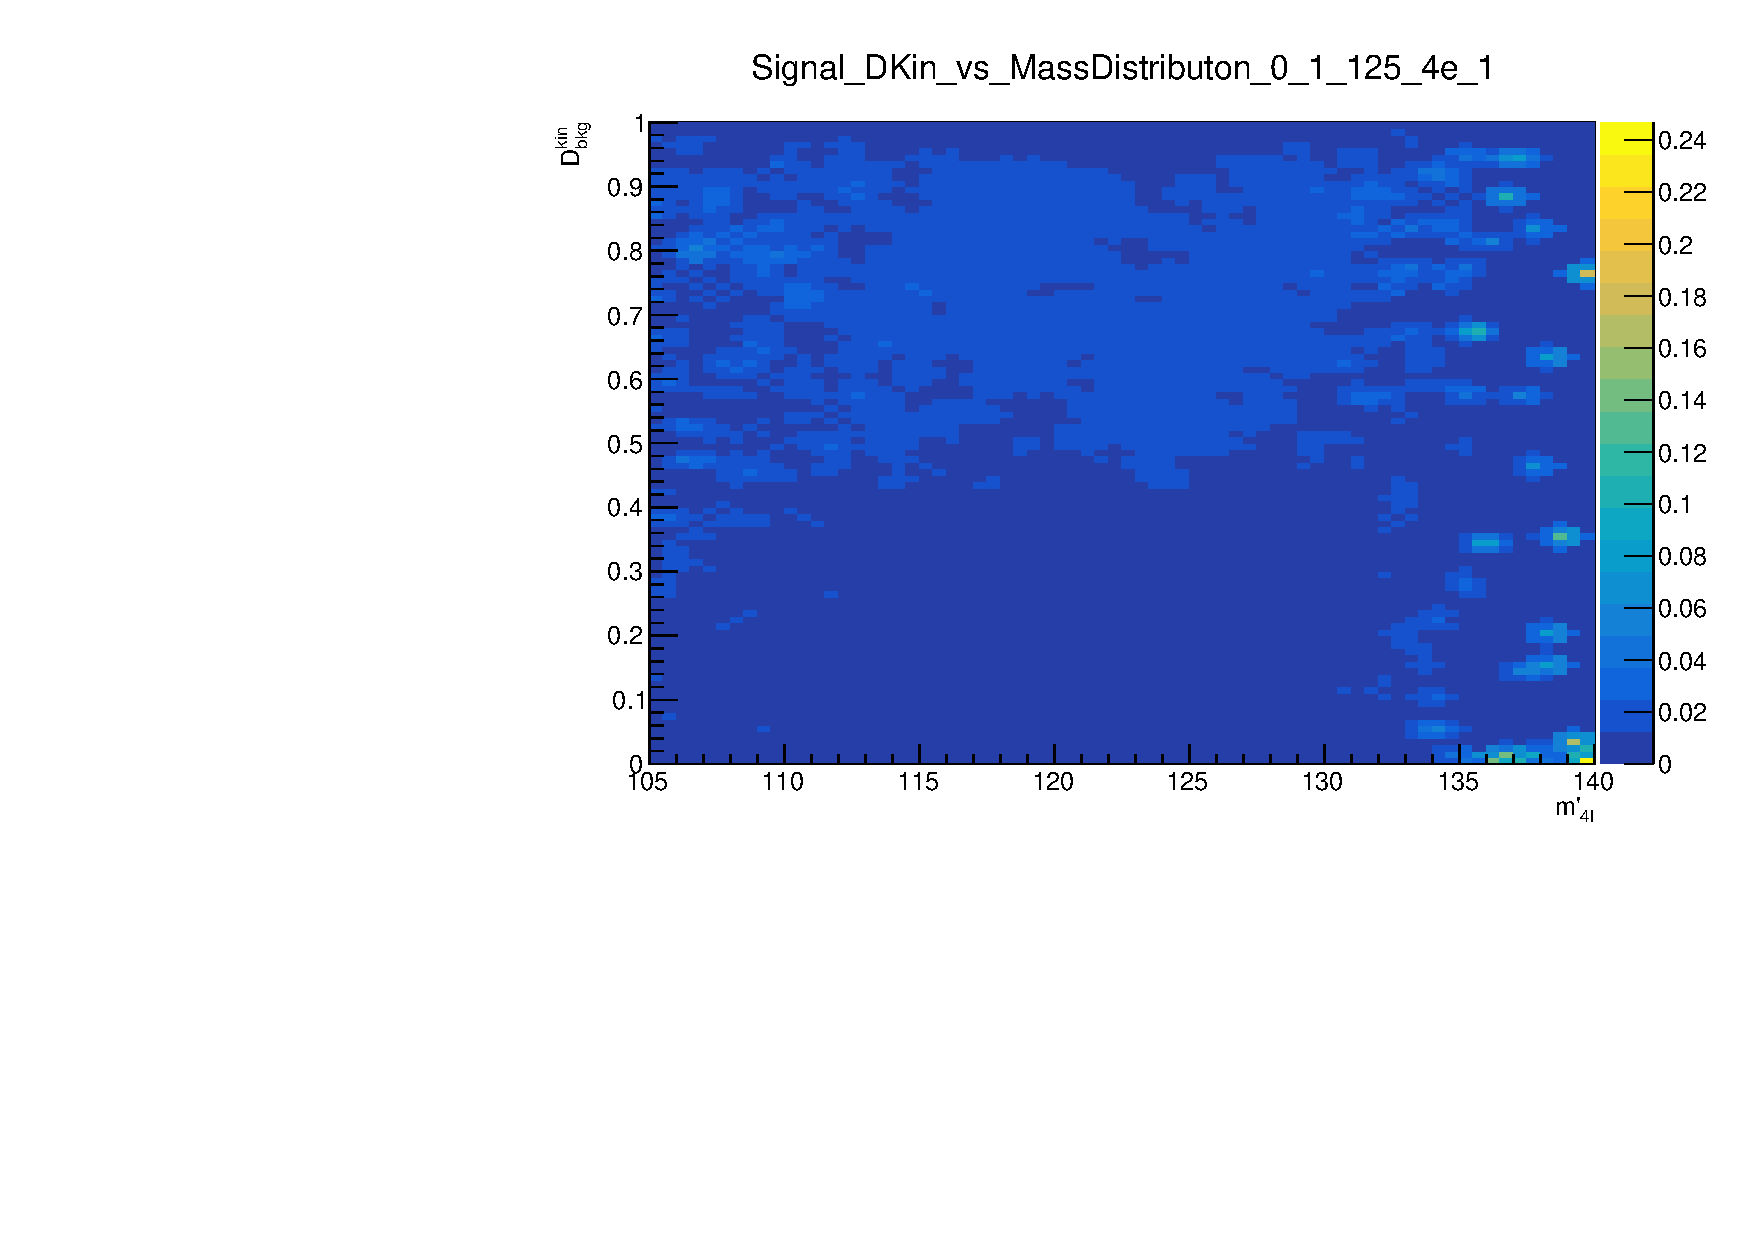
\includegraphics[width=0.45\textwidth]{../../higgsmassmeasurement/AN-19-248/Figures/BackDiscriminant/Dkin_vs_mass_4e_2018.pdf}
	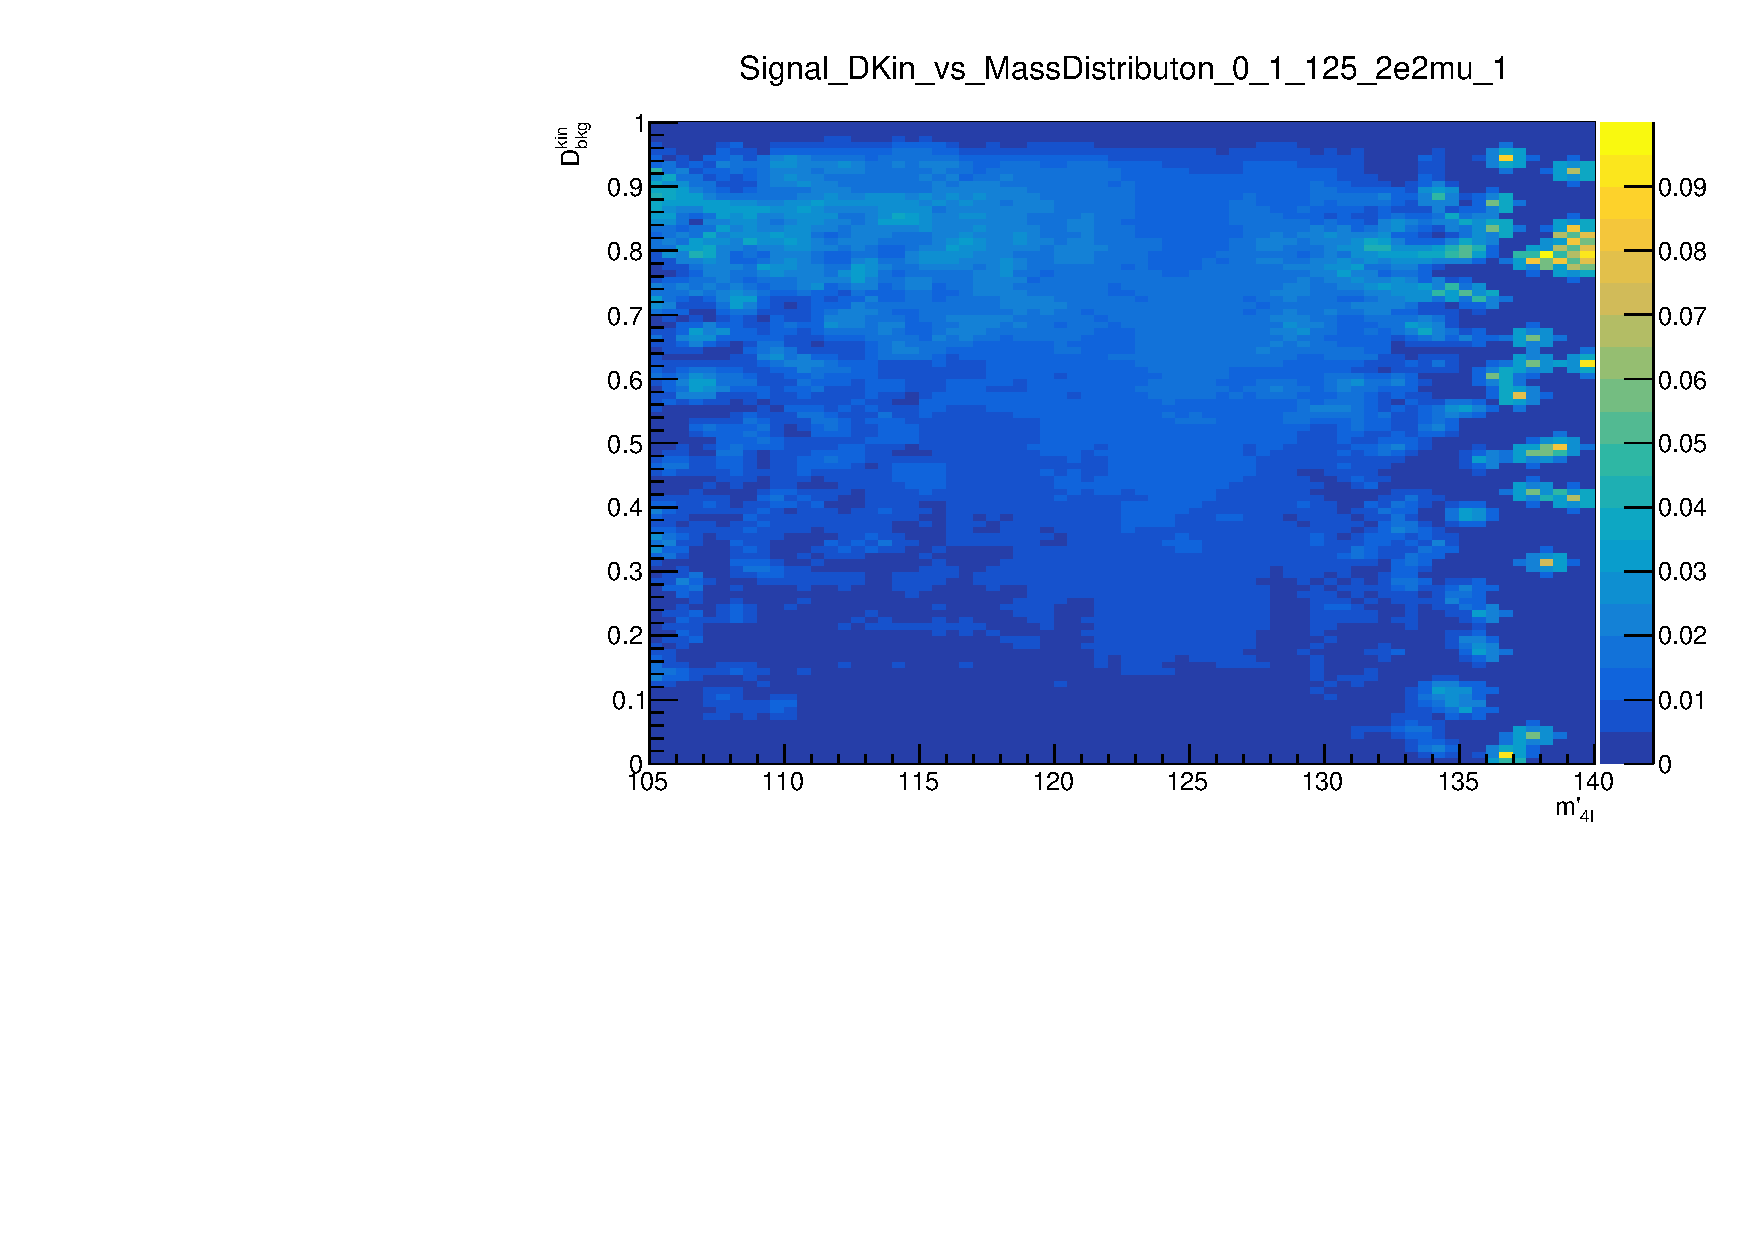
\includegraphics[width=0.45\textwidth]{../../higgsmassmeasurement/AN-19-248/Figures/BackDiscriminant/Dkin_vs_mass_2e2mu_2018.pdf}
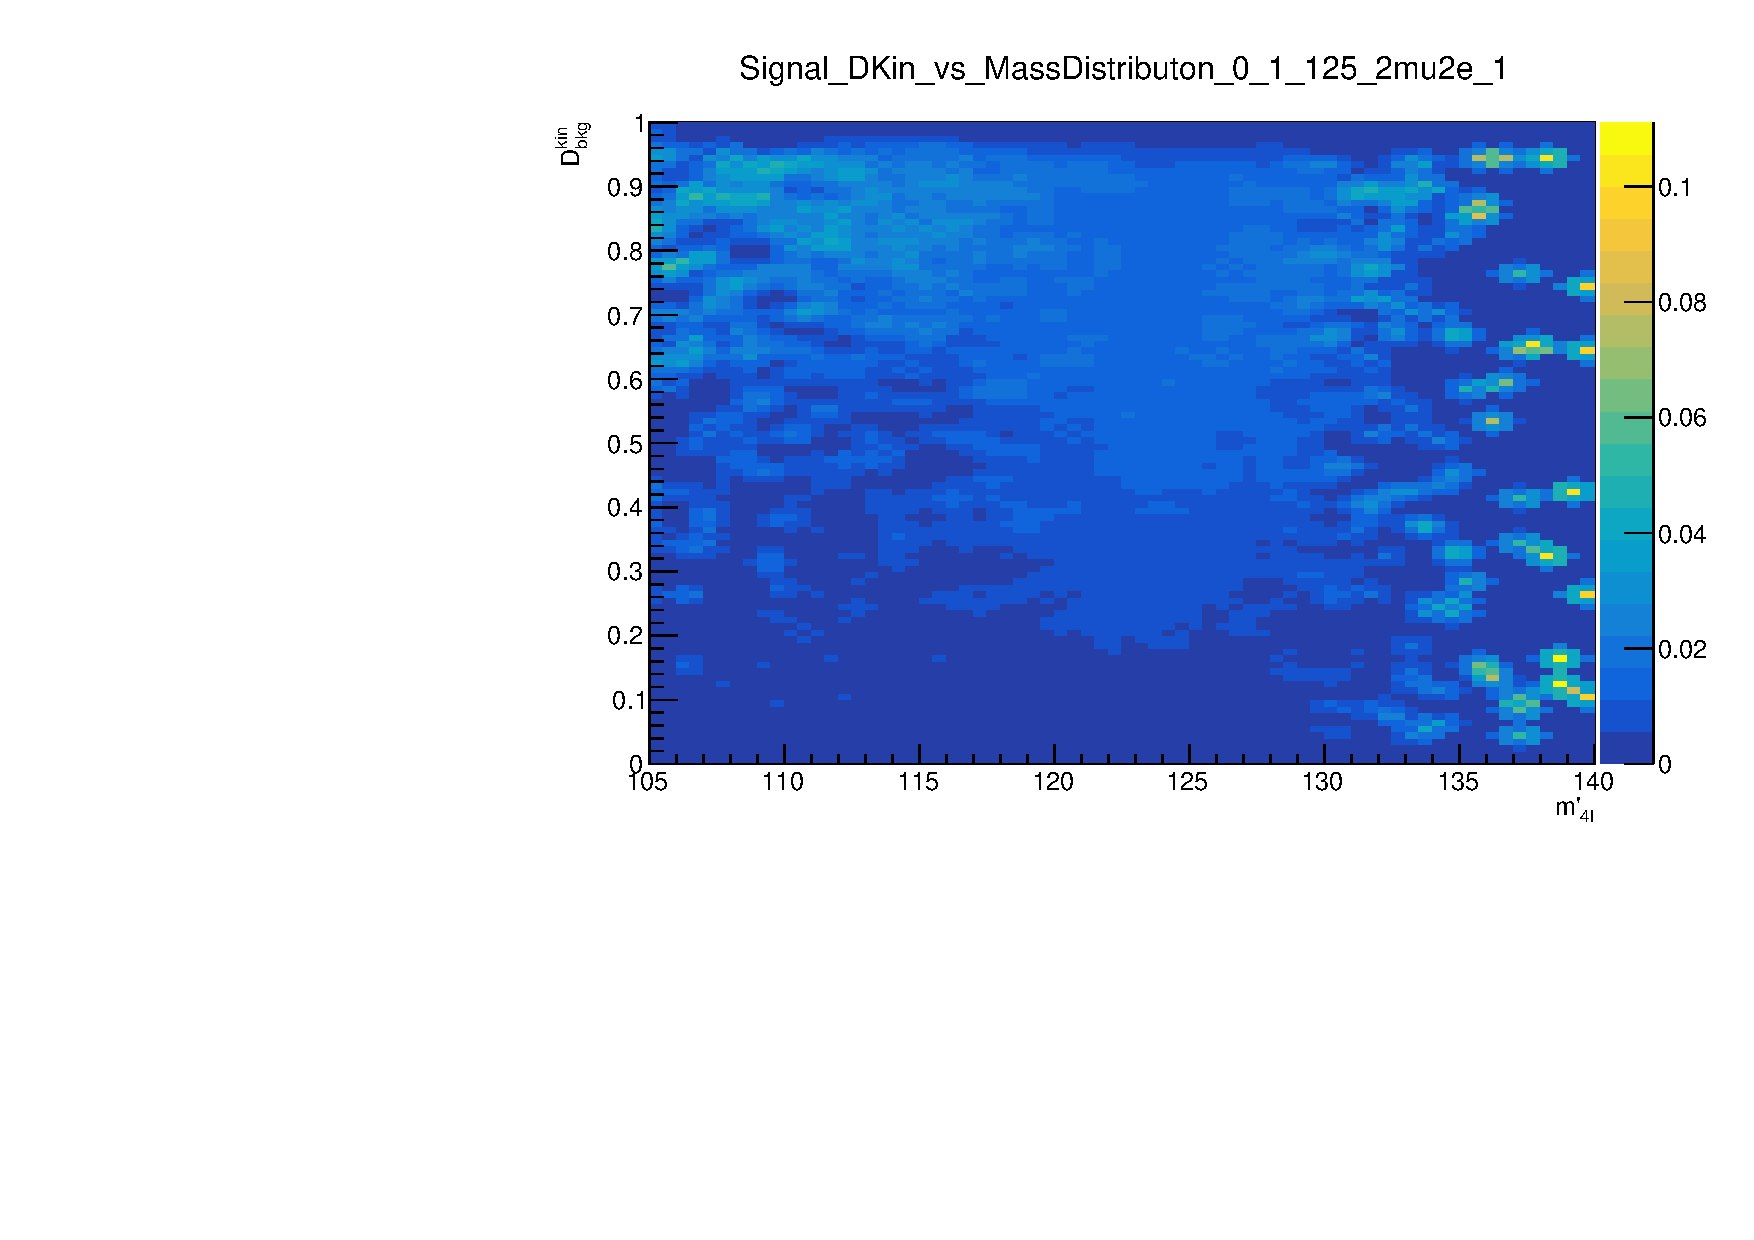
\includegraphics[width=0.45\textwidth]{../../higgsmassmeasurement/AN-19-248/Figures/BackDiscriminant/Dkin_vs_mass_2mu2e_2018.pdf}
\caption{
2D distribution for the inclusive relative mass error, for 2018, for different final state:
4$\mu$ on top left, 4e on top right, 2e2$\mu$ on bottom left and 2$\mu$2e on bottom right.}
\label{2D_distribution}
\end{center}
\end{figure}

As was the case for the signal processes, the backgrounds described in Sec: \ref{sec:BackgroundEstimation} are split into different relative mass error bins and are fitted using a 3rd order Bernstein polynomial function.

\subsection{Expected mass measurement uncertainties (MC)}
Expected results (in \MeV), when implementing the \Dkinbkg in the likelihood, 
are summarized in Tables~\ref{table:N2D_model_result} and~\ref{table:N2D_model_result_year}.
\begin{table}[ht]	
\begin{center}
	\topcaption
		[Expected Higgs boson mass uncertainty in the $4\ell$ final states, 
	with N-2D model]
		{Expected Higgs boson mass uncertainty in the $4\ell$ final states, 
	with N-2D model, compared with N-1D model only.
	All values are given in \MeV.  
	Statistical only results are considered at this stage of the analysis.
	}
	\begin{tabular}{ccccccc}
	\hline			
	Expected uncertainty	&	4$\mu$	&	4e	&	2e2$\mu$	&2$\mu$2e	& inclusive	&	 Rel. Improvement \\
	\hline			
	%	N-2$D'_{VXBS}$	&	\textbf{0.133}	&	\textbf{0.392}	&	\textbf{0.251}	&	\textbf{0.274}	&	\textbf{0.104}	\\
	%	N-1$D'_{VXBS}$	&	-0.143/0.145	&	-0.445/0.45	&	-0.274/0.276	&	-0.294/0.297	&	\textbf{0.113}	\\
	N-2$D'_{VXBS}$	&	143	&	440	&	266	&	300	&	112	&	-3\%	\\
	N-1$D'_{VXBS}$	&	148	&	465	&	271	&	310	&	116	&	-	\\
	\hline
	%	relative improvement	&	-	&	-	&	-	&	-	&	-	\\
	%	\hline
	\end{tabular}
	\label{table:N2D_model_result} 
\end{center}
\end{table}

\begin{table}[ht]	
\begin{center}
	\topcaption
		[Expected Higgs boson mass uncertainty in different years 
	with N-2D model]
		{Expected Higgs boson mass uncertainty in different years 
	with N-2D model, compared with N-1D model only.
	All values are given in \MeV.  
	Statistical only results are considered at this stage of the analysis.
	}
	\begin{tabular}{cccc}
	\hline			
	Expected uncertainty	&	2016	&	2017	&	2018	\\
	\hline			
	N-2$D'_{VXBS}$	&	221	&	206	&	167	\\
	N-1$D'_{VXBS}$	&	229	&	214	&	172	\\
	\hline
	\end{tabular}
	\label{table:N2D_model_result_year}
\end{center}
\end{table}
